\section{Motivación y contexto del proyecto}

Las obras pictóricas del patrimonio cultural, ya sean cuadros sobre lienzo o madera o murales de varios colores,
están formadas por distintas capas de materiales que reaccionan de forma continua con el ambiente~\citep{dePolo2021After}. 
Con el paso de los años, la técnica propia del artista, el tipo de componentes empleados y el impacto 
de factores como los cambios de temperatura, la humedad, la luz solar o los esfuerzos mecánicos 
terminan provocando un deterioro físico en la pieza. Entre los problemas más habituales 
destacan la aparición de grietas, el desprendimiento o la pérdida de partes de la pintura, 
la alteración del color y las deformaciones en la superficie o estructura que la sostiene~\citep{khalid2024review}.
El agrietamiento de la pintura no solo daña la apariencia del cuadro y reduce su valor histórico, 
sino que suele ser la causa directa de que el pigmento comience a descascararse, 
lo que en poco tiempo puede llevar a la pérdida definitiva de fragmentos originales~\citep{Degrigny2020WallPaintings}. 
Por otra parte, la forma en que se forman esas grietas funciona como un registro único del 
estado de conservación de la obra y de los daños que ha sufrido a lo largo de su historia. 
En la Figura \ref{fig:defectos} se muestran algunos ejemplos de defectos presentes en pinturas, que incluyen 
grietas, levantamiento de pintura, pérdida de pigmento y lesiones por impacto. Por este motivo, identificar estos fallos a tiempo y estudiarlos de manera constante resulta 
indispensable para proteger la obra y tomar decisiones acertadas antes de iniciar cualquier trabajo de restauración~\citep{VanVijle2025PaintingConservation}.


\begin{figure}[!hb]
    \centering
    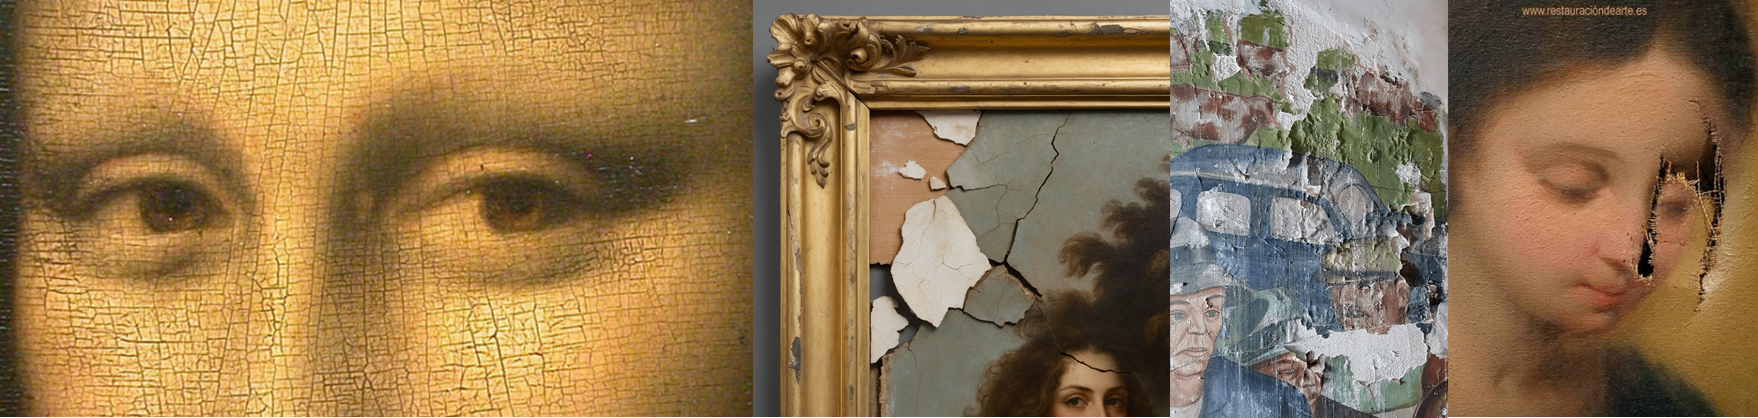
\includegraphics[width=0.99\textwidth]{defectos.png}
    \caption{\small Ejemplos de defectos presentes en pinturas. De izquiera a derecha se peude apreciar 
    grietas, levantamiento de pintura, pérdida de pigmento y lesiones por impacto.}
    \label{fig:defectos}
\end{figure}


Para identificar, delimitar y documentar los daños en obras pictóricas, se ha recurrido tradicionalmente a la inspección
visual de especialistas, complementada con imágenes científicas y fotografías con luz rasante, que permiten resaltar
irregularidades superficiales, levantamientos de pintura y deformaciones del soporte~\citep{Padfield2005PTM}.
Sin embargo, la interpretación de estas imágenes y la anotación manual de los deterioros pueden requerir un trabajo considerable
y dependen de la experiencia del conservador; además, la información registrada mediante fotografía con luz rasante
está condicionada por la posición de la iluminación, lo que dificulta la comparación entre campañas si no se mantiene
un protocolo reproducible~ \citep{VanVijle2025PaintingConservation}. Por otra parte, aunque determinados procedimientos de
caracterización material requieren la extracción de micromuestras, también existen técnicas químicas y
espectroscópicas no invasivas que permiten estudiar pigmentos, aglutinantes y productos de alteración directamente sobre
la obra ~\citep{Miliani2010MOLAB}. En este contexto, se han desarrollado métodos de adquisición
y análisis de imágenes para apoyar una documentación más reproducible y una evaluación cuantitativa de los deterioros.
Entre ellos, la fotogrametría, combinada con técnicas de escaneado tridimensional, permite documentar cambios geométricos
y seguir la evolución de redes de microgrietas, mientras que la visión por computador y el aprendizaje automático ofrecen
herramientas para detectar, segmentar y cartografiar grietas y pérdidas de pintura~\citep{Degrigny2020WallPaintings}.

El presente proyecto tiene finalidad desarrollar un \emph{framework} de análisis de imágenes que 
permita detectar y clasificar daños en pinturas. Las contribuciones principales al finalizar el proyecto son: 
i) una plataforma web que permita realizar el registro y análisis de daños en pinturas, ii) un conjunto de imágenes 
de obras pictóricas con daños, que sirva como base de datos para entrenar y evaluar los modelos de aprendizaje automático, y
iii) un modelo de visión por computador multimodal que combina información de diversar fuentes extraídas 
de las pinturas: imágenes RGB, térmicas y de fluorescencia, para detectar y clasificar los daños presentes 
en la obra.

%%%%%%%%%%%%%%%%%%%%%%%%%%%%%%%%%%%%%%%%%%%%%%%%%%%%%%%%%%%%%%%%%%%%%%%%%%%%%%%%%%%%%%%%%%%%%%%%%



\subsection{Objetivos del proyecto}

Para conseguir el objetivo principal del proyecto, se propone un pipeline que 
consta de tres etapas principales: a) Creación de la base de datos, b) Entrenamiento y evaluación 
del algoritmo, finalizando con c) Evaluación del framework. 


Para ello se definen el siguiente objetivo general:

\begin{itemize}
    \item OP: Desarrollar un framework de inteligencia artificial que permita detectar, identificar y clasificar daños 
    en pinturas de patrimonio cultural
\end{itemize}

A partir de este objetivo principal, se definen los siguientes objetivos específicos:

\begin{itemize}
    \item OE$_1$: Recopilación y etiquetado de daños en imágenes de pinturas patrimoniales basados en fotografías de 
    imágenes multimodales (luz visible - Infrarrojo - Ultravioleta - rayos X).
    \item OE$_2$: Implementación y validación del modelo computacional. 
    \item OE$_3$: Desarrollo del framework metodológico basado en inteligencia artificial.
\end{itemize}


%%%%%%%%%%%%%%%%%%%%%%%%%%%%%%%%%%%%%%%%%%%%%%%%%%%%%%%%%%%%%%%%%%%%%%%%%%%%%%%%%%%%%%%%%%%%%%%%%


\section{Detalle de la metodología}

En esta sección se describe el pipeline propuesto para la identificación de daños en pinturas patrimoniales.
Siguiendo la estructura de los objetivos planteados, el pipeline se divide en tres etapas principales: 
a) Edificación de la base de datos, b) Implementación y evaluación del algoritmo, finalizando con c) Desarrollo del framework. 
La Figura \ref{fig:metodologia} muestra un esquema general del pipeline propuesto, que se detalla a continuación.



\begin{figure}[!hb]
    \centering
    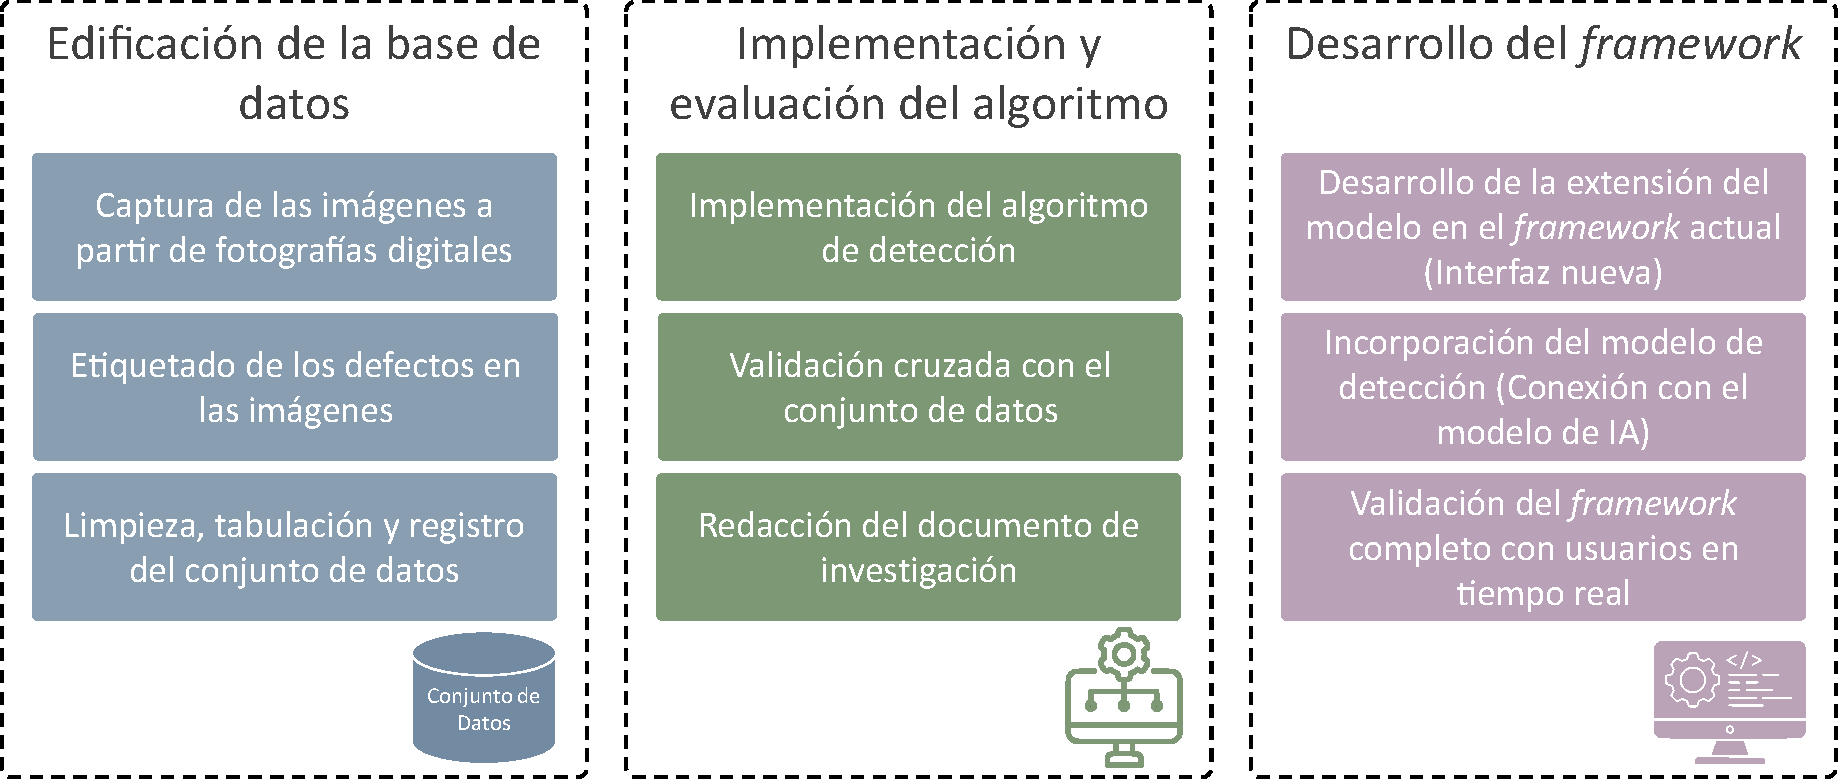
\includegraphics[width=0.9\textwidth]{figuras/Modelos.pdf}
    \caption{\small Esquema general del pipeline propuesto para la identificación de daños en pinturas patrimoniales.}
    \label{fig:metodologia}
\end{figure}


Cada una de las etapas del pipeline acude a conseguir cada uno de los objetivos específicos planteados en la sección anterior. 
En las siguientes subsecciones se describe cada una de las etapas del pipeline, detallando las tareas que se realizarán, 
los resultados esperados así como los responsables de cada tarea. Es importantes resaltar que los procesos que mostramos
en le Figura \ref{fig:metodologia} son los que se realizarán en el marco del proyecto, sin embargo, existen otros procesos 
administrativos y de gestión que no se muestran en la figura, pero que son necesarios para el correcto desarrollo del proyecto, 
éstos serán descritos en la sección de gestión del proyecto. Así mismo, el detalle de la tareas como la duración de cada una de ellas
estarán con maor detalle en la sección de Cronograma del proyecto~\ref{sec:cronograma}. 

\section{Edificación de la base de datos}

TODO amigos virreynales


\section{Implementación y evaluación del algoritmo}
En esta etapa se implementará un modelo de visión por computador basado en aprendizaje profundo que permita detectar y 
clasificar los daños presentes en las pinturas patrimoniales. Para ello, se utilizará la base de datos construida en la etapa anterior, 
que contendrá imágenes multimodales. Al igual que en la etapa anterior, detallaremos las tareas que se realizarán, sin embargo, 
también describiremos el modelo computacional que se implementará a partir de la investigación realizada en el marco del proyecto. 
El cual es una de las principales contribuciones del proyecto. Todas las tareas de esta etapa atienden al objetivo específico OE$_2$. 


\begin{itemize}
    \item Actores de esta etapa:

    \begin{itemize}
        \item Reponsable de toda la etapa: Prof. Aurea Soriano
        \item Investigadores: Prof. Aurea Soriano, Prof. Rensso Mora
        \item Investigador tesista: Estudiante Luis Lopez Chambi 
    \end{itemize}


        \item Lista de tareas a realizar en esta etapa:

    \begin{itemize}
        \item Tarea B$_1$: Levantamiento de estado del arte de modelos de visión por computador para la detección y clasificación de daños en pinturas. Responsables: Aurea Soriano y Luis Lopez Chambi.
        \item Tarea B$_2$: Implementación del algoritmo de detección y clasificación de daños. Responsables: Aurea Soriano, Rensso Mora, y Luis Lopez Chambi. 
        \item Tarea B$_3$: Evaluación del algoritmo propuesto. Responsables: Aurea Soriano y Luis Lopez Chambi.
        \item Tarea B$_4$: Redacción del documento científico. Responsables: Aurea Soriano y Luis Lopez Chambi.
        \item Tarea B$_5$: Redacción del informe. Responsables: Aurea Soriano y Luis Lopez Chambi. 
    \end{itemize}

\end{itemize}


\subsection{Tarea B$_1$: Levantamiento de estado del arte de modelos de visión por computador para la detección y clasificación de daños en pinturas}

La tarea B$_1$ tiene como objetivo realizar un levantamiento del estado del arte de modelos de visión por computador para la detección y clasificación de daños en pinturas.
Esta tarea se desarrolla desde el inicio de la participación del estudiante tesista en el proyecto y culmina al terminar la redacción del documento científico.
El resultado esperado de esta tarea es un documento que contenga el estado del arte de modelos de visión por computador para la detección y clasificación 
de daños en pinturas, esto es necesario para enriquecer la base de conocimiento del proyecto, resaltar las contribuciones de nuestro modelo contrastando
con los modelos ya existentes. De esta forma esta tarea atiende al objetivo específico OE$_2$.


\subsection{Tarea B$_2$: Implementación del algoritmo de detección y clasificación de daños}

La tarea B$_2$ tiene como objetivo implementar un modelo de visión por computador basado en aprendizaje profundo que permita detectar y clasificar 
los daños presentes en las pinturas patrimoniales. Esta tarea se desarrolla desde el inicio de la participación del estudiante tesista en el 
proyecto y culmina al terminar la redacción del documento científico. El resultado esperado de esta tarea es un modelo computacional que permita 
detectar y clasificar los daños presentes en las pinturas patrimoniales, esto es necesario para enriquecer la base de conocimiento del proyecto, 
resaltar las contribuciones de nuestro modelo contrastando con los modelos ya existentes. De esta forma esta tarea atiende al objetivo específico OE$_2$.

Si bien el modelo computacional es una de las principales contribuciones del proyecto, para la redacción del presente documento, se realizó un levantamiento
previo del estado del arte y se define el siguiente modelo computacional que será implementado en el marco del proyecto. 
El modelo propuesto es un modelo multimodal basado en aprendizaje profundo, que combina información de diversas fuentes extraídas de las pinturas: 
imágenes RGB, térmicas y de fluorescencia, para detectar y clasificar los daños presentes en la obra. La Figura \ref{fig:modelo} muestra la arquitectura 
propuesta para el modelo de detección y clasificación de daños en pinturas patrimoniales. Inspirados en los trabajos de fusión de características 
multimodal \citep{li2026video, tri_modal_fusion_transformers_conf}, el modelo propuesto utiliza la información de las imágenes multimodales para extraer 
características relevantes, esta fusión es necesaria ya que aunque las imágenes RGB proporcionan información visual detallada, las imágenes 
térmicas y de fluorescencia pueden revelar daños ocultos o alteraciones en la pintura que no son visibles a simple vista. 
Esta inforación de daños no  necesariamente coincide con la información de las imágenes RGB, por lo que la fusión de características permite al 
modelo aprender representaciones más completas y robustas de los daños presentes en las pinturas, y una fusión temprana no es suficiente para capturar 
la complejidad de los daños. En general la arquitectura se base en un decoder basado en swin transformer \citep{liu2021swin} y 
un encoder basado en DETR \citep{carion2020end}. 


\begin{figure}[!ht]
    \centering
    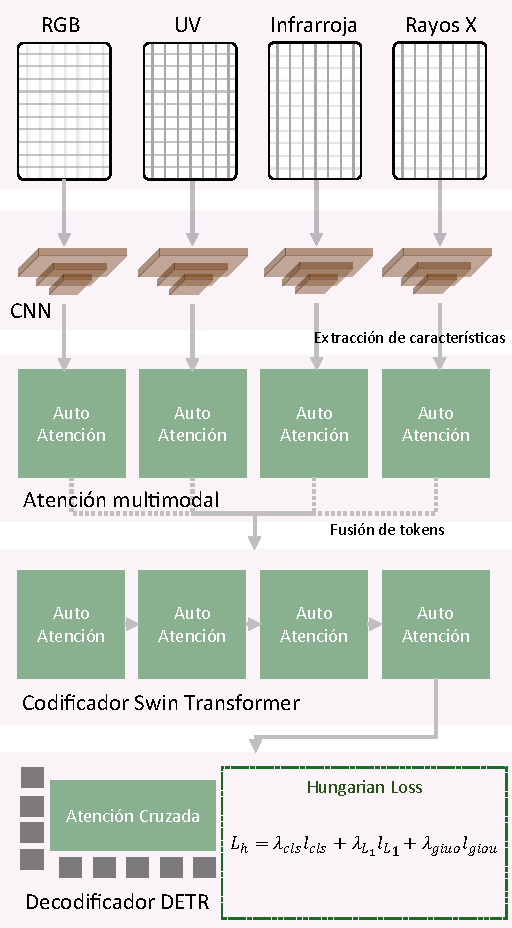
\includegraphics[width=0.35\textwidth]{figuras/Modelos2.pdf}
    \caption{\small Arquitectura propuesta para el modelo de detección y clasificación de daños en pinturas patrimoniales. Se divide en tres etapas: 
    a) Extracción de características, b) Fusión de características y c) Detección y clasificación.}
    \label{fig:modelo}
\end{figure}


\section{Cronograma del proyecto}\label{sec:cronograma}


